\begin{frame}[fragile]
  \frametitle{Our 1D Helmholtz problem}

  We consider the following problem,
  a simple yet telling example of a situation involving the Helmholtz equation:
  \vspace{0.6 cm}
  \begin{alertblock}{Our 1D Helmholtz problem}
    \vspace{-0.6cm}
    \begin{align}
      u'' + k^2 u &= 0 ~ ~ \text{in} ~ ~ ]0, 1[ \\
      u'(0) &= i k \\
      u'(1) &= i k u(1)
    \end{align}
    \vspace{-0.6cm}
  \end{alertblock}

\end{frame}


\subsection{PDE description}

\begin{frame}[fragile]
  \frametitle{About our problem}

  \begin{block}{Our 1D Helmholtz problem}
    \vspace{-0.6cm}
    \begin{align}
      \setcounter{equation}{0}
      u'' + k^2 u &= 0 ~ ~ \text{in} ~ ~ ]0, 1[ \\
      u'(0) &= i k \\
      u'(1) &= i k u(1)
    \end{align}
    \vspace{-0.6cm}
  \end{block}

  \begin{itemize}
    \item \( u \) is a 1D complex-valued function, at least two times derivable
    \item \(f = 0 \), so this problem "sourceless"/homogeneous
    \item (2), assigning a value to the derivative, is called a Neumann "flux" boundary condition.
    \item (3), establishing a linear relationship between the value and the derivative, is called a Robin "impedance" boundary condition.
  \end{itemize}

\end{frame}

\subsection{Exact solution}

\begin{frame}[fragile]
  \frametitle{The exact solution}

  The problem can be solved with linear PDE tools, yielding an unique solution:

  \begin{block}{The "Euler wave" exact solution}
    \vspace{-0.6cm}
    \begin{align*}
      \forall x \in [0, 1], ~ u(x) &= e^{ikx}
    \end{align*}
    \vspace{-0.6cm}
  \end{block}

  \begin{figure}
    \centering
    \subfloat[3D complex plot\label{fig:1a}]{
      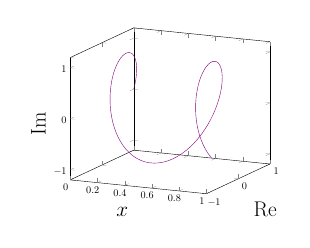
\begin{tikzpicture}[scale=0.37]
        \begin{axis}[
            view={25}{15},
            xlabel={\huge $x$},
            ylabel={\huge Re},
            zlabel={\huge Im},
        ]
          \addplot3+ [
              color=violet,
              domain=0:1,        % Changed: x from 0 to 1
              samples=100,       % Changed: more samples for smoothness
              samples y=1,
              mark=none,         % Added: removes the beads/markers
          ] (
              {x},
              {cos(deg(10*x))},  % Changed: x instead of \x, deg() for radians
              {sin(deg(10*x))}   % Changed: x instead of \x, deg() for radians
          );
      \end{axis}
    \end{tikzpicture}
    }
    \qquad
    \subfloat[Real part\label{fig:1b}]{
      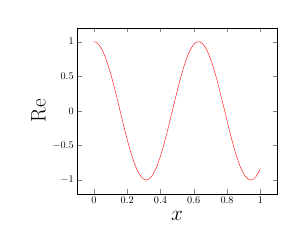
\begin{tikzpicture}[scale=0.37]
        \begin{axis}[
          xlabel={\huge $x$},
          ylabel={\huge Re},
        ]
          \addplot [
            color=red,
            domain=0:1,
            samples=100,
            mark=none,
          ] {
            cos(deg(10*x))
          };
        \end{axis}
      \end{tikzpicture}
    }
    \qquad
    \subfloat[Imaginary part\label{fig:1c}]{
      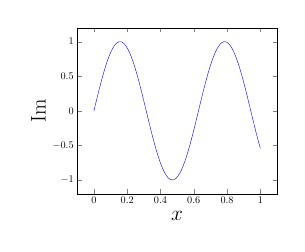
\begin{tikzpicture}[scale=0.37]
        \begin{axis}[
          xlabel={\huge $x$},
          ylabel={\huge Im}
        ]
          \addplot[
            color=blue,
            domain=0:1,
            samples=100,
            mark=none,
          ]{
            sin(deg(10*x))
          };
        \end{axis}
      \end{tikzpicture}
    }
  \label{fig:1}
  \caption{Exact solution with $k = 10$}
  \end{figure}

\end{frame}